\section{Lasso og dens generaliseringer}
\begin{frame}{Lasso og dens generaliseringer}
\begin{itemize}
\item Datasættet med 4 laggede værdier
\begin{itemize}
\item 126 variabler
\item Træningsmængde: 1. maj 1960 - 1. december 2005 (548 observationer)
\item Testmængde: 1. januar 2006 - 1. juli 2017 (139 observationer)
\end{itemize}
\item Lasso problemet og dens generaliseringer kan løses med coordinate descent algoritmen og LARS algoritmen
\begin{itemize}
\item Valg af tuning parameter
\begin{itemize}
\item Krydsvalidering
\item BIC
\end{itemize}
\end{itemize}
\end{itemize}
\end{frame}

\section{Coordinate descent}
\begin{frame}{Coordinate descent}
\begin{itemize}
\item Coordinate descent
\begin{itemize}
\item Algoritmen opdaterer fra $\boldsymbol \beta_t$ til  $\boldsymbol \beta_{t+1}$ ved at vælge en koefficient, som opdateres, og da udføres en univariat minimering. 
Koefficienten $k$ opdateres i iteration $t$, da er opdatering givet ved
\begin{align*}
\beta_k^{t+1} = \underset{\beta_k}{\arg\min} f\del{\beta_1^t,\dots, \beta_{k-1}^t, \beta_k, \beta_{k+1}^t, \dots, \beta_p^t },
\end{align*}
hvor 	$\beta_j^{t+1} = \beta^t_j$ for $j \neq k$
\begin{itemize}
\item Lasso, ridge regression, elastik net og adaptive lasso
\end{itemize}
\item Dette kan generaliseres til block coordinate descent, hvor prædiktorerne er opdelt i ikke-overlappende blocks, og da udføres en minimering over en enkelt block for hvert koordinat
\begin{itemize}
\item Group lasso
\end{itemize}
\end{itemize}
\end{itemize}
\end{frame}

\subsection{Krydsvalidering}
\begin{frame}{Coordinate descent}{Krydsvalidering}
\begin{itemize}
\item Fitter en model for hver $\lambda$
\begin{itemize}
\item $\lambda_{\min}$: mindste gennemsnitlige krydsvalideringsfejl
\item $\lambda_{1\text{sd}}$: største værdi af $\lambda$, således at fejlen stadig er inden for en standard afvigelse af minimum 
\end{itemize}
\item Elastisk net og adaptive lasso har to tuning parametre
\begin{itemize}
\item Elastisk net: $\alpha \in [0,1]$ 
\begin{itemize}
\item Elastisk net (CV): $\alpha = 1$
\end{itemize}
\item Adaptive lasso: $\gamma \in \cbr{0.5, 1, 2}$
\begin{itemize}
\item Adaptive lasso med OLS vægte (CV): $\gamma = 0.5$
\item Adaptive lasso med lasso vægte (CV): $\gamma = 0.5$
\end{itemize}
\end{itemize}
\end{itemize}
\end{frame}

\begin{frame}{Coordinate descent}{Krydsvalidering}
\begin{table}
\center
\begin{tabular}{cccc | cccccc}
\toprule
 &  \multicolumn{3}{c}{Lasso} &  \multicolumn{3}{c}{Ridge}  \\ \midrule
 & værdi & MSE & p & 	værdi & MSE & p \\
 $\lambda_{\min}$ &0.0014& 0.0019 & 20 	& 0.0123 &  0.0049 & 122 \\ 
 $\lambda_{1 \text{sd}}$ & 0.0027 & 0.0020 & 15 & 0.0148 & 0.0051 & 122  \\ \bottomrule \toprule
  &  \multicolumn{3}{c}{Elastic Net}  &  \multicolumn{3}{c}{Group Lasso}  \\ \midrule
 & værdi & MSE & p & værdi & MSE & p \\
 $\lambda_{\min}$ & 0.0014 & 0.0020 & 23 & 0.0003 & 0.0023  & 122\\
  $\lambda_{1\text{sd}}$ & 0.0027 & 0.0021 & 15 & 0.0005 & 0.0024 & 122 \\  \bottomrule \toprule
 &  \multicolumn{3}{c}{Adaptive lasso m. OLS vægte}  &  \multicolumn{3}{c}{Adaptive lasso m. lasso vægte}  \\ \midrule
  & værdi & MSE & p & værdi & MSE & p \\
 $\lambda_{\min}$  & 0.0868 & 0.0018 & 2 & 0.0034 & 0.0018 & 4   \\
 $\lambda_{1\text{sd}}$ & 0.4222 & 0.0018 & 2 & 0.0085 & 0.0019 & 4  \\ \bottomrule
 \end{tabular}
\caption{Tabellen viser $\lambda$ værdierne fundet udfra krydsvalidering, samt krydsvalideringsfejl, som er målt i MSE og antallet af parameter.} \label{tab:cv_tab}
\end{table}

\end{frame}


\begin{frame}{Coordinate descent}{Krydsvalidering}
\begin{itemize}
\item Group lasso (CV)
\begin{itemize}
\item Ikke valgte variable tilhører alle gruppe 5 (penge og kredit)
\end{itemize}
\item Adaptive lasso med OLS vægte (CV) og adaptive lasso med lasso vægte (CV)
\begin{itemize}
\item Vælger variablerne \textcolor{blue3}{CLF16OV}: Civilarbejdsstyrke,   \textcolor{blue3}{CE16OV}: Civilbeskæftigelse   
\item Konsistent i variableudvælgelse
\end{itemize}
\end{itemize}
\end{frame}


\begin{frame}{Coordinate descent}{Krydsvalidering}
\begin{itemize}
\item 1000 bootstrap relisationer af $\widehat{\vbeta} \del{\lambda_{1\text{sd}}}$
\end{itemize}
\begin{figure}[!htb]
        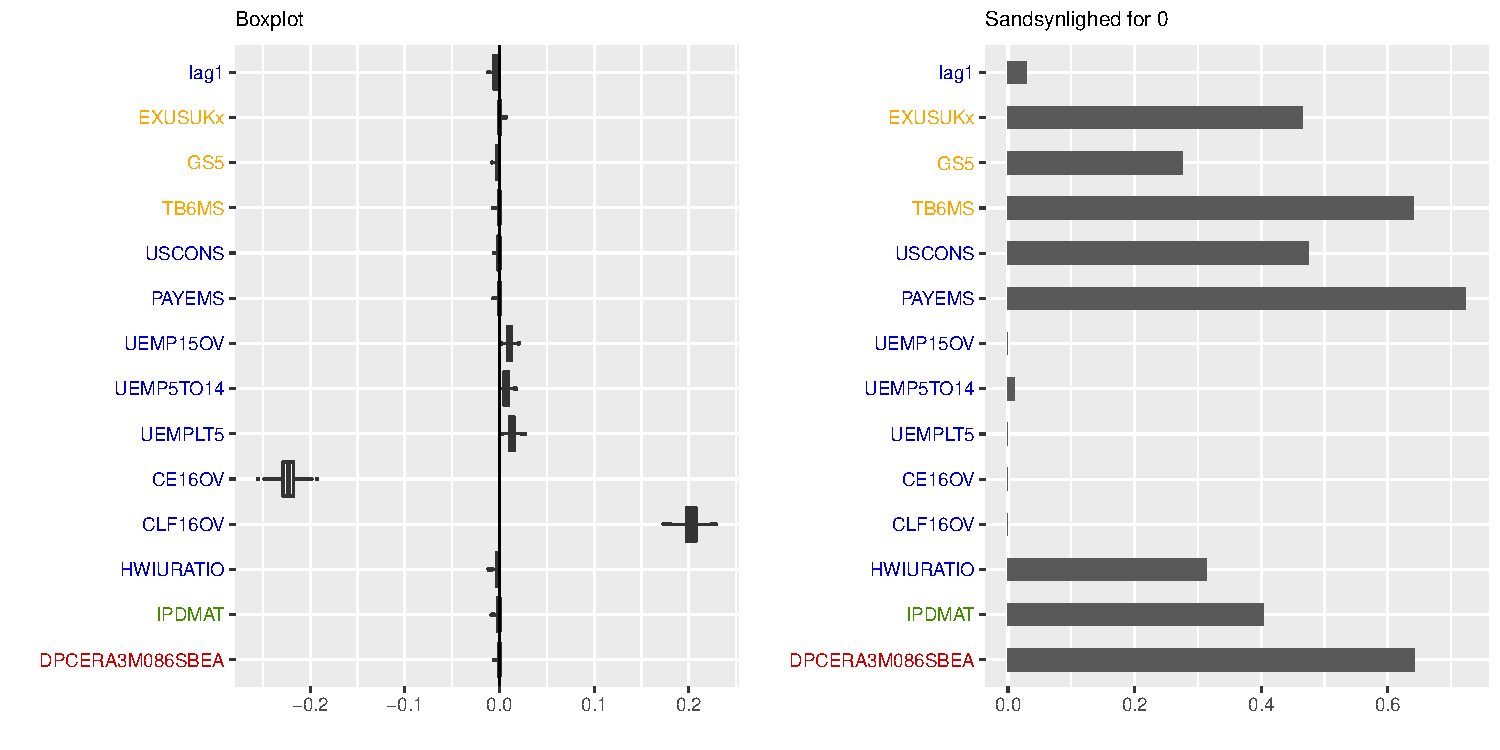
\includegraphics[width=1\linewidth, height=0.7\textheight]{slides/boxplot_lasso_coord_kryds.pdf}
% \caption{Til venstre vises et boxplot af 1000 bootstrap realisationer af $\widehat{\beta}^{\text{lasso}} \del{\lambda_{\text{1sd}}} $. Plottet til højre illustrerer andelen af bootstrap realisationer, hvor parameter estimaterne er præcis lig nul.}
\end{figure}
  %         
\end{frame}

\begin{frame}{Coordinate descent}{Krydsvalidering}
\begin{itemize}
\item Polyede variableudvælgelse 
\end{itemize}
%\begin{table}[ht] 
%\centering 
%%\scalebox{0.8}{
%\begin{tabular}{lcccc}
%\toprule
%Prædiktor & Koefficient & Z-score & \(p\)-værdi & Konfidensinterval \\
%\midrule
%\textcolor{red3}{DPCERA3M086SBEA} & -0.002 & -1.365 &  0.666  &  [-0.009, 0.026]  \\
%\textcolor{chartreuse4}{IPDMAT} & -0.003  &-1.113  & 0.268  &  [-0.012, 0.006]  \\
%\textcolor{blue3}{HWIURATIO}  & 0.002 &  0.718 &  0.197 &   [-0.003,  0.014]   \\
%\textcolor{blue3}{CLF16OV} & 0.243 & 36.668  & 0   &  [0.232,  0.259]\\
%\textcolor{blue3}{CE16OV} &  -0.266 & -37.390 &  0  &  [-0.280 , -0.254]\\
%\textcolor{blue3}{UEMPLT5} & 0.001  & 0.241  & 0.402  &  [-0.005  ,  0.008 ] \\
%\textcolor{blue3}{UEMP5TO14} & 0.000 & -0.118 &  0.429  & [ -0.007  ,  0.004 ]\\
%\textcolor{blue3}{UEMP15OV}& 0.004  & 1.593  & 0.056 &   [ 0.000  ,  0.009] \\
%\textcolor{blue3}{PAYEMS} & 0.001 &  0.273  & 0.223  &  [-0.007  ,  0.029 ] \\
%\textcolor{blue3}{USCONS} & -0.002 & -0.883 &  0.569 &  [ -0.009  ,  0.016] \\
%\textcolor{orange}{TB6MS} & -0.001 & -0.480 &  0.682 &  [ -0.009  ,  0.026 ] \\
%\textcolor{orange}{GS5} & -0.003 & -1.131  & 0.219  & [ -0.025  , 0.007 ] \\
%\textcolor{orange}{EXUSUKx} & 0.003 &  1.306 &  0.872 &  [ -0.072 , 0.003 ] \\
%\textcolor{blue3}{lag 1} & -0.009 & -4.067  & 0.003 &  [ -0.013, -0.004] \\
%\bottomrule
%\end{tabular}  
%%}
%\caption{\(p\)-værdier og konfidensintervaller for variablerne udvalgt af lasso. Den estimeres standard afvigelse er \(0.043\), og resultaterne er for \(\widehat{\lambda} = \widehat{\lambda}_\text{1sd} \cdot 548 \approx 1.823\) med \(\alpha = 0.1\).} \label{tab:fixedLassoInf}
%\end{table} 

\begin{table}[ht] 
\centering 
\scalebox{0.7}{
\begin{tabular}{lcccccc}
\toprule
Prædiktor &Koefficient & Z-score &  \(p\)-værdi & Konfidensinterval &  $\sbr{\pazocal{V}^-,\pazocal{V}^+}$  \\
\midrule
 \textcolor{red3}{DPCERA3M086SBEA}   & $-0.002$   &$-1.362$  &  0.671   & $\sbr{-0.009   ,  0.027} $  & $\sbr{0.002,0.004}$ \\
\textcolor{chartreuse4}{IPDMAT} & $-0.003$   &$-1.113  $&  0.265    & $\sbr{-0.012   ,  0.006 } $   & $\sbr{0.000,0.004} $\\   
\textcolor{blue3}{HWIURATIO}     & 0.002  &  0.717  & 0.199    & $\sbr{-0.003   , 0.014 } $ &$\sbr{ -0.002,0.004} $\\
\textcolor{blue3}{CLF16OV}  & 0.243  & 36.671 & 0  & $\sbr{  0.232 ,   0.259  } $    &  $\sbr{0.203,0.252} $ \\ 
\textcolor{blue3}{CE16OV}  & $-0.266$ &$ -37.393$    &  0   & $\sbr{-0.280  , -0.254} $ & $\sbr{0.230,0.278} $ \\  
\textcolor{blue3}{UEMPLT5}& 0.001    &0.240     &0.402  &$\sbr{-0.005  ,  0.008 } $    & $\sbr{-0.011,0.009 } $\\
\textcolor{blue3}{UEMP5TO14}  &0.000 &  $-0.118$   &  0.430     &$\sbr{-0.006  ,  0.004 } $  & $\sbr{ -0.010,0.005} $  \\
 \textcolor{blue3}{UEMP15OV}  & 0.004  &  1.593   &0.056  &   $\sbr{0.000   ,  0.009  } $ &  $\sbr{-0.006,0.013} $ \\
\textcolor{blue3}{PAYEMS} & 0.001   & 0.280   & 0.219    & $\sbr{-0.007  ,  0.030      } $ &  $\sbr{-0.002,0.002} $\\
\textcolor{blue3}{USCONS} & $-0.002$  & $-0.883$   & 0.566    &$\sbr{ -0.009    , 0.016  } $ & $\sbr{0.001,0.004} $\\
\textcolor{orange}{TB6MS} & $- 0.001$  & $-0.480$     &0.682  &  $\sbr{ -0.009    , 0.026  } $ &$\sbr{ 0.000,0.004} $\\
\textcolor{orange}{GS5}  & $-0.003$   &$-1.130$ &0.219     &$\sbr{-0.025    ,0.007   } $    & $\sbr{0.001, 0.004} $\\
\textcolor{orange}{EXUSUKx}  & 0.003  &  1.307   &0.870    &$\sbr{ -0.071  ,  0.003     } $ &  $\sbr{0.002,0.006} $\\
\textcolor{blue3}{lag 1}  & $-0.009$  &  $-4.065$  &   0.003   &  $\sbr{-0.013 ,  -0.004      } $   &$\sbr{0.005,0.015} $\\
\bottomrule
\end{tabular}  
}
\caption{Koefficienter, \(Z\)-scores, \(p\)-værdier, konfidensintervaller og trunkeret intervaller for lasso$_{TG}$ (CV). Den estimeres standard afvigelse er \(0.043\), og resultaterne er for \(\lambda_{TG} = \lambda_\text{1sd} \cdot 548 \approx 1.823\) med \(\alpha = 0.1\).} \label{tab:fixedLassoInf}
\end{table} 
\end{frame}

\subsection{BIC}
\begin{frame}{Coordinate descent}{BIC}
\begin{itemize}
\item Fitter en værdi for hver $\lambda$
\begin{itemize}
\item $\lambda_{\text{BIC}}$: mindste BIC
\end{itemize}
\item Elastik net og adaptive lasso har to tuning parametre 
\begin{itemize}
\item Elastisk net: $\alpha \in [0,1]$ 
\begin{itemize}
\item Elastisk net (BIC): $\alpha = 1$
\end{itemize}
\item Adaptive lasso: $\gamma \in \cbr{0.5, 1, 2}$
\begin{itemize}
\item Adaptive lasso med OLS vægte (BIC): $\gamma = 2$
\item Adaptive lasso med lasso vægte (BIC): $\gamma = 0.5$
\end{itemize}
\end{itemize}
\end{itemize}
\end{frame}


\begin{frame}{Coordinate descent}{BIC}
%\begin{table}
%\center
%\begin{tabular}{lccc} 
%\toprule
%& \multicolumn{1}{c}{Lasso} & \multicolumn{1}{c}{Ridge regression}  &  \multicolumn{1}{c}{Group lasso}\\ \midrule
%$\log \del{\widehat{\lambda}_\text{BIC}}$ & $-6.2639$ & $-4.4730$  & $-7.2876$ \\
%$p$ & 17 & 126 & 99 \\
%BIC & $-6.1608 $& $-3.3230$ & $-5.0721$  \\
%Adj. R$^2$ & 94.23 \% & 86.98  \%   & 92.11 \%  \\ \bottomrule \toprule
%& Adap. lasso m. OLS vægte & Adap. lasso m. lasso vægte \\ \midrule
%$\log \del{ \widehat{\lambda}_\text{BIC}}$ &  $-2.6212$& $-1.8390$ \\
%$p$ & 2&2 \\
%BIC &  $-6.3153$&$-6.3142$ \\
%Adj. R$^2$ & 94.28 \% &  94.28 \% \\ \bottomrule
% \end{tabular}
%\caption{Logaritmen af $\widehat{\lambda}_\text{BIC}$, antallet af parametre, BIC og adjusted R$^2$ for lasso og dens generaliseringer.} \label{tab:bic_lambda}
%\end{table}

\begin{table}
\center
\begin{tabular}{lcccc  | lccccc} 
\toprule
 \multicolumn{5}{c}{Lasso} && \multicolumn{5}{c}{Ridge regression}  \\ \midrule
& $\log \del{\widehat{\lambda}_\text{BIC}}$  & BIC & $p$ & R$^2_{\text{adj}}$ && & $\log \del{\widehat{\lambda}_\text{BIC}}$  &  BIC & $p$ &R$^2_{\text{adj}}$  \\
$\widehat{\lambda}_\text{BIC} $&  $-6.2639$ & $-6.1608$ & 17 &  94.23 \% && $\widehat{\lambda}_\text{BIC} $ & $-4.4730$ & $-3.3230$ &  126 & 86.98 \% \\ \bottomrule \toprule 
 \multicolumn{5}{c}{Group lasso} && \multicolumn{5}{c}{Adap. lasso m. OLS vægte}  \\ \midrule
& $\log \del{\widehat{\lambda}_\text{BIC}}$  & BIC & $p$ &R$^2_{\text{adj}}$ && & $\log \del{\widehat{\lambda}_\text{BIC}}$  &  BIC & $p$ &R$^2_{\text{adj}}$   \\
$\widehat{\lambda}_\text{BIC}$ & $-7.2876$ &  $-5.0721$ &99  & 92.11\% &&  $\widehat{\lambda}_\text{BIC}$ & $-2.6212$ &  $-6.3153$  & 2 & $94.28 \%$ \\ \bottomrule \toprule 
 \multicolumn{5}{c}{Adap. lasso m. lasso vægte}  \\
& $\log \del{\widehat{\lambda}_\text{BIC}}$  & BIC & $p$ & R$^2_{\text{adj}}$\\
 $\widehat{\lambda}_\text{BIC}  $&  	$-1.8390$ & $-6.3142$  & 2& 94.28\% \\ \cmidrule{1-5}
 \end{tabular}
\caption{Logaritmen af $\widehat{\lambda}_\text{BIC}$, antallet af parametre, BIC og adjusted R$^2$ for lasso og dens generaliseringer.} \label{tab:bic_lambda}
\end{table}
\end{frame}


\begin{frame}{Coordinate descent}{BIC}
\begin{itemize}
\item Group lasso (CV)
\begin{itemize}
\item Ikke valgte variable 
\begin{itemize}
\item 11 / 14 variable fra penge og kredit
\item 12 /20 variable fra priser
\item 3/30 variable fra arbejdsmarked
\end{itemize} 
\end{itemize}
\item Adaptive lasso med OLS vægte (CV)
\begin{itemize}
\item Vælger variablerne \textcolor{blue3}{CLF16OV}: Civilarbejdsstyrke,   \textcolor{blue3}{CE16OV}: Civilbeskæftigelse   
\item Konsistent i variableudvælgelse
\end{itemize}
\item Adaptive lasso med lasso vægte (CV)
\begin{itemize}
\item Vælger variablerne \textcolor{blue3}{CLF16OV}: Civilarbejdsstyrke,   \textcolor{blue3}{CE16OV}: Civilbeskæftigelse og \textcolor{blue3}{lag1}:Tidligere værdi af arbejdsløshedsrate
\item Konsistent i variableudvælgelse
\end{itemize}
\end{itemize}
\end{frame}

\begin{frame}{Coordinate descent}{BIC}
\begin{figure}[!htb]
        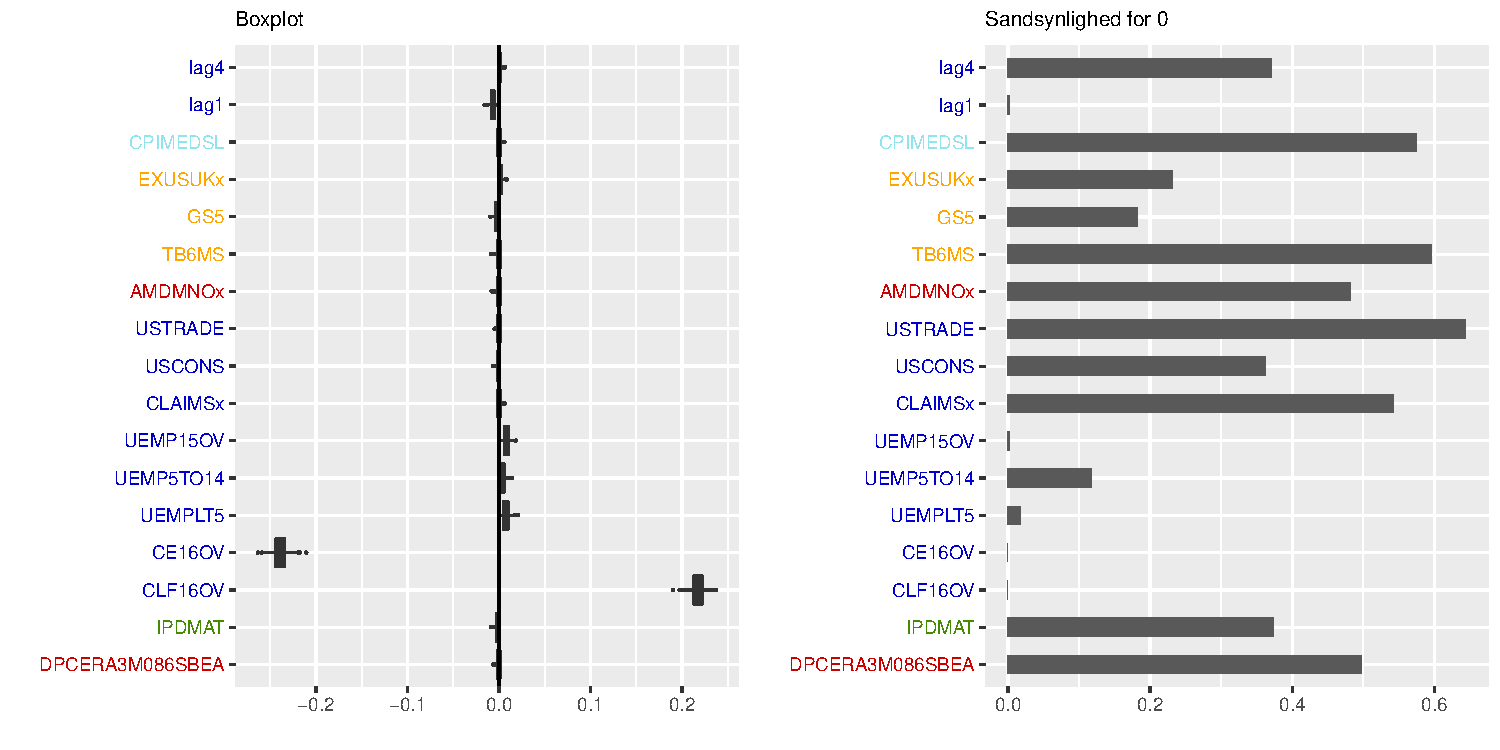
\includegraphics[width=1\linewidth, height=0.7\textheight]{slides/boxplot_lasso_coord_bic.pdf}
\end{figure}
  %          \caption{Til venstre vises et boxplot af 1000 bootstrap realisationer af $\widehat{\tbeta}^{\text{lasso}} \del{\lambda_{\text{1sd}}} $. Plottet til højre illustrerer andelen af bootstrap realisationer, hvor parameter estimaterne er præcis lig nul.}
\end{frame}

\begin{frame}{Coordinate descent}{BIC}
\begin{itemize}
\item Polyede variableudvælgelse 
\end{itemize}
\begin{table}[h] 
\centering 
\scalebox{0.8}{
\begin{tabular}{llllllll}
\toprule
Prædiktor & Koefficient & Z-score & \(p\)-værdi & lowConfPt & UpConfPt & LowTailArea & UpTailArea\\
\midrule
\textcolor{red3}{DPCERA3M086SBEA}  & -0.002  &-0.960   &0.093  &   -0.071  &  0.003      & 0.000   &  0.050 \\
\textcolor{chartreuse4}{IPDMAT} &-0.002 & -0.680 &  0.159  &  -0.032 &   0.005     &  0.050    &  0.049 \\
\textcolor{blue3}{CLF16OV} & 0.241  &36.686  & 0.000 &    0.235   & 0.350    &   0.050  &    0.050 \\
\textcolor{blue3}{CE160V} &-0.264& -37.339   &0.000  &  -0.455  & -0.260   &    0.050   &   0.050 \\
\textcolor{blue3}{UEMPLT5}  & 0.000 &  0.027 &  0.777   & -0.029    &0.005    &   0.000  &     0.048 \\
\textcolor{blue3}{UEMP5TO14} & -0.001  & -0.266 & 0.599  & -0.007   &  0.014    &   0.050 &      0.050 \\
\textcolor{blue3}{UEMP15OV} &0.004  & 1.299  & 0.249   & -0.005   & 0.008  &     0.050     & 0.049 \\
\textcolor{blue3}{CLAIMSx} & 0.001 &  0.387  & 0.689   & -0.030   & 0.011    &  0.050     & 0.050 \\
\textcolor{blue3}{USCONS}  & -0.001  &  -0.591   &  0.100  &    -0.088  &     0.004  &      0.050  &       0.050 \\
\textcolor{blue3}{USTRADE}  & 0.000  & -0.118  &  0.988     & 0.007     &  Inf     &   0.050  &     0.000\\
\textcolor{red3}{AMDMNOx} &-0.002 &  -0.813 &  0.641  &  -0.008  &  0.020   &    0.049      &0.050 \\
\textcolor{orange}{TB6MS}&-0.001  &-0.415  & 0.677   & -0.008  &  0.023   &    0.049   &   0.000 \\
\textcolor{orange}{GS5} &-0.003 & -1.207  & 0.144    &-0.032  &  0.005      & 0.050    &  0.050 \\
\textcolor{orange}{EXUSUKx} & 0.003  & 1.449   &0.303   & -0.007   & 0.012      & 0.050    &  0.050 \\
\textcolor{cadetblue2}{CPIMEDSL}  &0.002 &  0.855 &  0.865&    -0.054 &   0.003&       0.050    &  0.050 \\
\textcolor{blue3}{lag1} & -0.010&  -4.362 &  0.499  &  -0.011   & 0.033   &    0.050  &    0.050 \\
\textcolor{blue3}{lag4}  & 0.002 &   1.106   & 0.311    & -0.014 &    0.028 &       0.036 &      0.050 \\
\bottomrule
\end{tabular}  
}
\caption{\(p\)-værdier og konfidensintervaller for variablerne udvalgt af lasso med BIC. Den estimeres standard afvigelse er 0.043, og resultaterne er for $\lambda \approx 1.0432$  med \(\alpha = 0.1\).} \label{tab:fixedLassoInf_bic}
\end{table} 
\end{frame}
